\documentclass[11pt]{article}
\usepackage{euscript}

\usepackage{amsmath}
\usepackage{amsthm}
\usepackage{amssymb}
\usepackage{mathtools}
\DeclarePairedDelimiter{\ceil}{\lceil}{\rceil}
\usepackage{epsfig}
\usepackage{xspace}
\usepackage{color}
\usepackage{url}
\usepackage{enumerate}
\usepackage{listings}

\usepackage{float}

%%%%%%%  For drawing trees  %%%%%%%%%
\usepackage{tikz}
\usetikzlibrary{calc, shapes, backgrounds}

%%%%%%%%%%%%%%%%%%%%%%%%%%%%%%%%%
\setlength{\textheight}{9in}
\setlength{\topmargin}{-0.600in}
\setlength{\headheight}{0.2in}
\setlength{\headsep}{0.250in}
\setlength{\footskip}{0.5in}
\flushbottom
\setlength{\textwidth}{6.5in}
\setlength{\oddsidemargin}{0in}
\setlength{\evensidemargin}{0in}
\setlength{\columnsep}{2pc}
\setlength{\parindent}{1em}
%%%%%%%%%%%%%%%%%%%%%%%%%%%%%%%%%

\newcommand{\eps}{\varepsilon}

\renewcommand{\c}[1]{\ensuremath{\EuScript{#1}}}
\renewcommand{\b}[1]{\ensuremath{\mathbb{#1}}}
\newcommand{\s}[1]{\textsf{#1}}

\newcommand{\E}{\textbf{\textsf{E}}}
\renewcommand{\Pr}{\textbf{\textsf{Pr}}}


\title{Asmt 3: Clustering}
\author{Yulong Liang (u1143816)}

\begin{document}
\maketitle

\section{Hierarchical Clustering (20 points)}

\paragraph{A: (20 points)} 
The results of Hierarchical Clustering are as follows,\\

\textbf{Single-Link measurement}
\begin{figure}[H]
\centering{
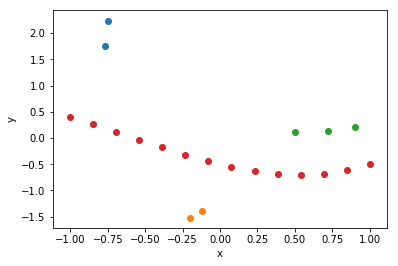
\includegraphics[width=.5\linewidth]{hc_1.png}
}
\caption{Hierarchical Clustering with Single-Link measurement}
\label{fig:name}
\end{figure}

\textbf{Complete-Link measurement}
\begin{figure}[H]
\centering{
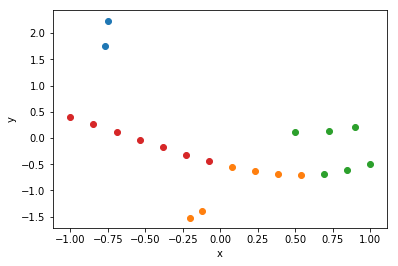
\includegraphics[width=.5\linewidth]{hc_2.png}
}
\caption{Hierarchical Clustering with Complete-Link measurement}
\label{fig:name}
\end{figure}

\newpage

\textbf{Mean-Link measurement}
\begin{figure}[H]
\centering{
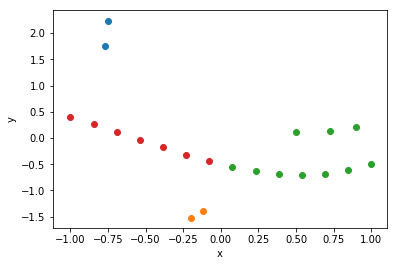
\includegraphics[width=.5\linewidth]{hc_3.png}
}
\caption{Hierarchical Clustering with Mean-Link measurement}
\label{fig:name}
\end{figure}

\subparagraph{Result Analysis}
In this case, \textbf{Single-Link} did the best job. It sucessfully clustered the points so that within each cluster, the points follow the same pattern.
\subparagraph{Complexity Analysis}
Among the three measurements, \textbf{Mean-Link} is the easiest to compute, although for this small case, Mean-Link took the longest time of $0.06s$.\\
For Single-Link and Complete-Link, the calculation of distance requires $O(m\cdot n)$ time, where $m, n$ are the numbers of elements in $S_1, S_2$ respectively. Whereas, Mean-Link takes $O(m+n)$ to compute the mean points and the distance between. Moreover, we can use vector calculation with \texttt{Numpy} to dramatically reduce the computation complexity.

\section{Assignment-Based Clustering (40 points)}

\paragraph{A: (20 points)}
 
For \texttt{Gonzalez} Algorithm, the centers are as follows,
$$(-2.7694973, 2.6778586) \quad (-2, 14) \quad (-0.4032861, -5.4479696)$$
The result is shown in the following graph,
\begin{figure}[H]
\centering{
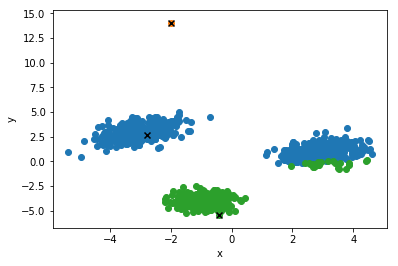
\includegraphics[width=.5\linewidth]{gonzalez.png}
}
\caption{\texttt{Gonzalez} Algorithm}
\label{fig:name}
\end{figure}
\begin{itemize}
\item 3-center cost:
$$Cost=max_{x\in X}\mathbf{d}(x, \phi_C(x))=7.6422437929188733$$
\item 3-means cost:
$$Cost=\sqrt{\frac{1}{|X|}\sum_{x\in X}(\mathbf{d}(x, \phi_C(x)))^2}=3.69933167681$$
\end{itemize}

For \texttt{k-Means++} Algorithm, the cumulative density function is as follows,
\begin{figure}[H]
\centering{
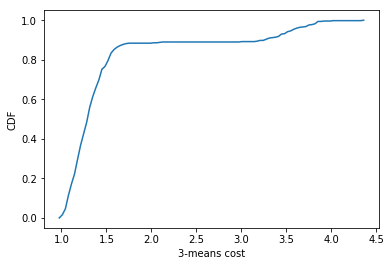
\includegraphics[width=.5\linewidth]{kmeanspp.png}
}
\caption{CDF of \texttt{k-Means++} Algorithm}
\label{fig:name}
\end{figure}
\begin{itemize}
\item Fraction of same results: \textbf{0\%}\\
I ran the algorithm for 500 times. None of the cluster results were the same as the result from \texttt{Gonzalez}. Most of the results looked like the following graph,
\begin{figure}[H]
\centering{
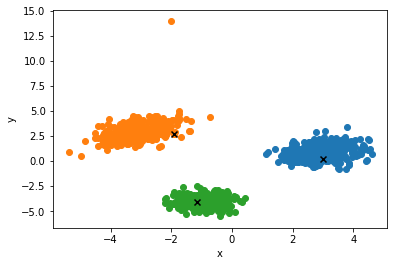
\includegraphics[width=.5\linewidth]{kmeanspp2.png}
}
\caption{\texttt{k-Means++} Algorithm}
\label{fig:name}
\end{figure}
\end{itemize}

\newpage

\paragraph{B: (20 points)}
For initialization with points indexed $\{1,2,3\}$, the final subset is as follows,
\begin{figure}[H]
\centering{
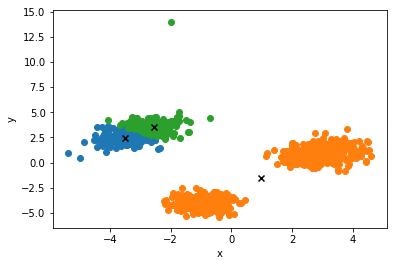
\includegraphics[width=.5\linewidth]{kmeans1.png}
}
\caption{\texttt{k-Means} Algorithm initialized with points indexed $\{1,2,3\}$}
\label{fig:name}
\end{figure}
\begin{itemize}
\item 3-means cost:
$$Cost=\sqrt{\frac{1}{|X|}\sum_{x\in X}(\mathbf{d}(x, \phi_C(x)))^2}=2.74960790413928$$
\end{itemize}

For initialization with the outputs of \texttt{Gonzalez}, the final subset is as follows,
\begin{figure}[H]
\centering{
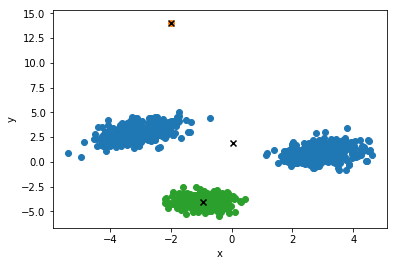
\includegraphics[width=.5\linewidth]{kmeans2.png}
}
\caption{\texttt{k-Means} Algorithm initialized with \texttt{Gonzalez}}
\label{fig:name}
\end{figure}
\begin{itemize}
\item 3-means cost:
$$Cost=\sqrt{\frac{1}{|X|}\sum_{x\in X}(\mathbf{d}(x, \phi_C(x)))^2}=2.7142310473085742$$
\end{itemize}

For initialization with the outputs of \texttt{k-Means++}, the cumulative density function is as follows,
\begin{figure}[H]
\centering{
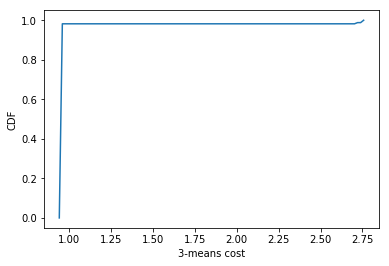
\includegraphics[width=.5\linewidth]{kmeans3.png}
}
\caption{CDF of \texttt{k-Means++} Algorithm}
\label{fig:name}
\end{figure}

\begin{itemize}
\item Fraction of same results : \textbf{88.2\%}\\
I ran the algorithm for 500 times. 88.2\% of the \texttt{k-Means} cluster outputs were the same as the inputs, i.e., the output from \texttt{k-Means++}. However, the output of \texttt{k-Means} typically has centers which are located at the center of each cluster, which is different from that of \texttt{k-Means++}. Most of the results looked like the following graph,
\begin{figure}[H]
\centering{
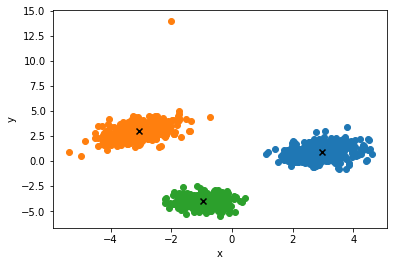
\includegraphics[width=.5\linewidth]{kmeans4.png}
}
\caption{\texttt{k-Means++} Algorithm}
\label{fig:name}
\end{figure}
\end{itemize}

\section{High-dimensional Distances (15 points)}
\begin{enumerate}
\item for $d=2$\\
$$vol(box(d,r))=(2r)^d=(2r)^2=4r^2$$
$$vol(B(d,cr))=\frac{\pi^{d/2}}{\Gamma(d/2+1)}(cr)^d=\frac{\pi}{\Gamma(2)}(cr)^2=\pi c^2r^2$$
\begin{align*}
vol(box(d,r))&=vol(B(d,cr))\\
4r^2&=\pi c^2r^2\\
c&={\sqrt{\frac{4}{\pi}}}\approx1.1283791670955126
\end{align*}

\item for $d=3$\\
$$vol(box(d,r))=(2r)^d=(2r)^3=8r^3$$
$$vol(B(d,cr))=\frac{\pi^{d/2}}{\Gamma(d/2+1)}(cr)^d=\frac{\pi^{3/2}}{\Gamma(2.5)}c^3r^3$$
\begin{align*}
vol(box(d,r))&=vol(B(d,cr))\\
8r^3&=\frac{\pi^{3/2}}{\Gamma(2.5)}c^3r^3\\
c&=\sqrt[3]{\frac{8\Gamma(2.5)}{\pi^{3/2}}}\approx1.2407009817988
\end{align*}

\item for $d=4$\\
$$vol(box(d,r))=(2r)^d=(2r)^4=16r^4$$
$$vol(B(d,cr))=\frac{\pi^{d/2}}{\Gamma(d/2+1)}(cr)^d=\frac{\pi^2}{\Gamma(3)}c^4r^4$$
\begin{align*}
vol(box(d,r))&=vol(B(d,cr))\\
16r^4&=\frac{\pi^2}{\Gamma(3)}c^4r^4\\
c&=\sqrt[4]{\frac{16\Gamma(3)}{\pi^2}}\approx1.3418765339308278
\end{align*}

\item as a function of d (for large d), restricting to even values of d
\begin{align*}
vol(box(d,r))&=vol(B(d,cr))\\
(2r)^d&=\frac{\pi^{d/2}}{\Gamma(d/2+1)}(cr)^d\\
c&=\Big[\frac{2^d\cdot\Gamma(d/2+1)}{\pi^{d/2}}\Big]^{1/d}
\end{align*}

\item Plot the expansion factor c up to d = 20
\begin{figure}[H]
\centering{
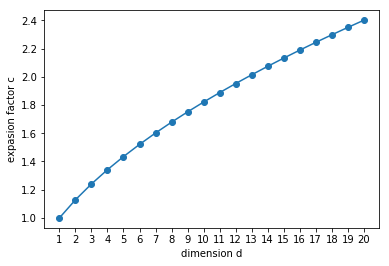
\includegraphics[width=.5\linewidth]{df.png}
}
\caption{Expansion Factor for $d\in[1,20]$}
\label{fig:name}
\end{figure}
\end{enumerate}

\section{k-Median Clustering (25 points)}

\paragraph{A: (20 points)}
The set of centers is as follows,
$$(-0.0035486, -0.0044096, 1.0163268, -0.0030803, -0.0093929)$$
$$(1.0047017, 0.0156167, 0.0081674, 0.0027186, -0.0036095)$$
$$(-0.0017825, 0.4591598, 0.0104942, 0.5182719, 0.0028535)$$
$$(0.9820007, 1.9938338, 0.0010286, -0.0058505, 0.9928755)$$
The k-Median Cost is,
$$Cost_1(P, C)=\frac{1}{|P|}\sum_{p\in P}\mathbf{d}(p, \phi_C(p))=0.4194209920788442$$
The approach to find the centers is as follows,
\begin{itemize}
\item Choose 4 points in P arbitrarily as initial centers,
\item Assign each point in P to the nearest center to form clusters,
\item Recompute the median of each cluster, which is the point with each feature value the median of the corresponding feature value for all the points,
\item Repeat \textbf{Step 2-3} until the set of centers remains unchanged,
\item Run \textbf{Step 1-4} several times to find the global minimum. 
\end{itemize}

\paragraph{B: (5 points)}
The set of centers is as follows,
$$(1.0047017, 0.0156167, 0.0081674, 0.0027186, -0.0036095)$$
$$(0.0045376, -0.0071952, 0.0064950, 0.9955599, 0.0071472)$$
$$(0.9820007, 1.9938338, 0.0010286, -0.0058505, 0.9928755)$$
$$(-0.0059094, 1.0028380, 0.0139273, 0.0032831, -0.0012778)$$
$$(-0.0035486, -0.0044096, 1.0163268, -0.0030803, -0.0093929)$$
The k-Median Cost is,
$$Cost_1(P, C)=\frac{1}{|P|}\sum_{p\in P}\mathbf{d}(p, \phi_C(p))=0.21145289311509274$$

\newpage

\section{Appendix: Codes}
\begin{lstlisting}[language=Python]
import pandas as pd
import numpy as np
from matplotlib import pyplot as plt
import time

c1df = pd.read_csv('C1.txt', sep='\t', index_col=0, header=None)
c1df.head()

def euclidean_dist(x, y):
    return np.linalg.norm(x - y)

def single_link(x, y):
    minValue = np.inf
    for i in x:
        for j in y:
            dist = euclidean_dist(i, j)
            if (dist < minValue):
                minValue = dist
    return minValue

def complete_link(x, y):
    maxValue = -1
    for i in x:
        for j in y:
            dist = euclidean_dist(i, j)
            if (dist > maxValue):
                maxValue = dist
    return maxValue

def mean_link(x, y):
    x_mean = np.array(x).mean(axis=0)
    y_mean = np.array(y).mean(axis=0)
    return euclidean_dist(x_mean, y_mean)

clusters = []
for i in range(c1df.shape[0]):
    cluster = []
    cluster.append(np.array(c1df.iloc[i]))
    clusters.append(cluster)

start = time.time()
while len(clusters) > 4:
    k = len(clusters)
    minDist = np.inf
    minI = -1
    minJ = -1
    for i in range(k):
        for j in range(i+1,k):
            dist = mean_link(clusters[i], clusters[j])
            if (dist < minDist):
                minDist = dist
                minI = i
                minJ = j
    for p in clusters[minJ]:
        clusters[minI].append(p)
    del clusters[minJ]
print(time.time()-start)

for cluster in clusters:
    points = np.array(cluster)
    plt.scatter(points[:,0], points[:,1])
plt.xlabel('x')
plt.ylabel('y')
plt.show()

for cluster in clusters:
    newcluster = set()
    for point in cluster:
        newcluster.add(tuple(point))
    print(newcluster)
    
import pandas as pd
import numpy as np
from matplotlib import pyplot as plt

c2df = pd.read_csv('C2.txt', sep='\t', header=None, index_col=0)
c2df.head()

def dist(x, y):
    return np.linalg.norm(x - y)

def gonzalez(x, k):
    n = x.shape[0]
    c = []
    c.append(x[0])
    fi = [0] * n
    
    for i in range(1, k):
        maxDist = 0
        c.append(x[0])
        for j in range(n):
            currDist = dist(x[j], c[fi[j]])
            if (currDist > maxDist):
                maxDist = currDist
                c[i] = x[j]
        for j in range(n):
            if (dist(x[j], c[fi[j]]) > dist(x[j], c[i])):
                fi[j] = i
    return c, fi

def center_cost(x, c, fi):
    n = x.shape[0]
    
    maxDist = 0
    maxI = -1
    maxJ = -1
    for i in set(fi):
        center = c[i]
        for j in range(n):
            if (fi[j] != i):
                break
            currDist = dist(center, x[j])
            if (currDist > maxDist):
                maxDist = currDist
                maxI = i
                maxJ = j
    return maxDist

def mean_cost(x, c, fi):
    n = x.shape[0]
    lst = []
    for i in range(n):
        lst.append(x[i] - c[fi[i]])
    mat = np.array(lst)
    return np.linalg.norm(mat) / n ** (1/2)

def mean_cost2(x, c, fi):
    n = x.shape[0]
    ssd = 0
    for i in range(n):
        ssd += dist(x[i], c[fi[i]]) ** 2
    return (ssd / n)**(1/2)

c2 = c2df.as_matrix()
c_gonzalez, fi_gonzalez = gonzalez(c2, 3)

result_gonzalez = c2df.copy()
result_gonzalez['cluster'] = np.array(fi_gonzalez)

for i in set(fi_gonzalez):
    cluster = result_gonzalez[result_gonzalez['cluster'] == i]
    plt.scatter(cluster.iloc[:,0], cluster.iloc[:,1])
plt.scatter(x=np.array(c_gonzalez)[:,0], y=np.array(c_gonzalez)[:,1], marker='x', c='black')
plt.xlabel('x')
plt.ylabel('y')
plt.show()

center_cost(c2, c_gonzalez, fi_gonzalez)
mean_cost(c2, c_gonzalez, fi_gonzalez)
mean_cost2(c2, c_gonzalez, fi_gonzalez)

def kmeanspp(x, k):
    n = x.shape[0]
    c = []
    c.append(x[np.random.randint(0,n)])
    fi = [0] * n
    for i in range(1, k):
        lst = []
        for j in range(n):
            lst.append(dist(x[j], c[fi[j]]) ** 2)
        arr = np.array(lst)
        prob = arr / arr.sum()
        idx = np.random.choice(np.arange(n), p=prob)
        c.append(x[idx])
        for j in range(n):
            if (dist(x[j], c[fi[j]]) > dist(x[j], c[i])):
                fi[j] = i
    return c, fi

c_kmeanspp, fi_kmeanspp = kmeanspp(c2, 3)

while True:
    c_kmeanspp, fi_kmeanspp = kmeanspp(c2, 3)
    cost = mean_cost(c2, c_kmeanspp, fi_kmeanspp)
    if (cost < 3):
        break

result_kmeanspp = c2df.copy()
result_kmeanspp['cluster'] = np.array(fi_kmeanspp)

for i in set(fi_kmeanspp):
    cluster = result_kmeanspp[result_kmeanspp['cluster'] == i]
    plt.scatter(cluster.iloc[:,0], cluster.iloc[:,1])
plt.scatter(x=np.array(c_kmeanspp)[:,0], y=np.array(c_kmeanspp)[:,1], marker='x', c='black')
plt.xlabel('x')
plt.ylabel('y')
plt.show()

kmpp_c = []
kmpp_fi = []
kmpp_cost = []
for i in range(500):
    c_kmeanspp, fi_kmeanspp = kmeanspp(c2, 3)
    kmpp_c.append(c_kmeanspp)
    kmpp_fi.append(fi_kmeanspp)
    kmpp_cost.append(mean_cost(c2, c_kmeanspp, fi_kmeanspp))

a = plt.hist(kmpp_cost, cumulative=True, bins=100, normed=1)

x = a[1]
y = np.concatenate((np.array([0]), a[0]))
plt.plot(x, y)
plt.xlabel('3-means cost')
plt.ylabel('CDF')
plt.show()

def find_center(c, p):
    minDist = np.inf
    minIdx = -1
    for i in range(len(c)):
        currDist = dist(c[i], p)
        if (currDist < minDist):
            minDist = currDist
            minIdx = i
    return minIdx

def kmeans(x, k, c=[]):
    n = x.shape[0]
    
    if (len(c) == 0):
        for i in range(k):
            c.append(x[i])
    fi = [-1] * n
    
    while True:
        for i in range(n):
            fi[i] = find_center(c, x[i])
        newc = []
        for j in range(k):
            idxs = [idx for idx in range(n) if fi[idx] == j]
            newc.append(x[idxs].mean(axis=0))
        if (np.array_equal(np.array(newc), np.array(c))):
            break
        else:
            c = newc
    
    return c, fi

c_kmeans1, fi_kmeans1 = kmeans(c2, 3)

result_kmeans1 = c2df.copy()
result_kmeans1['cluster'] = np.array(fi_kmeans1)

for i in set(fi_kmeans1):
    cluster = result_kmeans1[result_kmeans1['cluster'] == i]
    plt.scatter(cluster.iloc[:,0], cluster.iloc[:,1])
plt.scatter(x=np.array(c_kmeans1)[:,0], y=np.array(c_kmeans1)[:,1], marker='x', c='black')
plt.xlabel('x')
plt.ylabel('y')
plt.show()

mean_cost(c2, c_kmeans1, fi_kmeans1)

c_kmeans2, fi_kmeans2 = kmeans(c2, 3, c_gonzalez)

result_kmeans2 = c2df.copy()
result_kmeans2['cluster'] = np.array(fi_kmeans2)

for i in set(fi_kmeans2):
    cluster = result_kmeans2[result_kmeans2['cluster'] == i]
    plt.scatter(cluster.iloc[:,0], cluster.iloc[:,1])
plt.scatter(x=np.array(c_kmeans2)[:,0], y=np.array(c_kmeans2)[:,1], marker='x', c='black')
plt.xlabel('x')
plt.ylabel('y')
plt.show()

mean_cost(c2, c_kmeans2, fi_kmeans2)

c_kmeans3, fi_kmeans3 = kmeans(c2, 3, c_kmeanspp)

result_kmeans3 = c2df.copy()
result_kmeans3['cluster'] = np.array(fi_kmeans3)

for i in set(fi_kmeans3):
    cluster = result_kmeans3[result_kmeans3['cluster'] == i]
    plt.scatter(cluster.iloc[:,0], cluster.iloc[:,1])
plt.scatter(x=np.array(c_kmeans3)[:,0], y=np.array(c_kmeans3)[:,1], marker='x', c='black')
plt.xlabel('x')
plt.ylabel('y')
plt.show()

mean_cost(c2, c_kmeans3, fi_kmeans3)

total = len(kmpp_c)
same = 0

km_cost = []
for i in range(total):
    c_km, fi_km = kmeans(c2, 3, kmpp_c[i])
    km_cost.append(mean_cost(c2, c_km, fi_km))
    if (sum(kmpp_fi[i]) == sum(fi_km)):
        same += 1

same/total

b = plt.hist(km_cost, cumulative=True, bins=100, normed=1)

x = b[1]
y = np.concatenate((np.array([0]), b[0]))
plt.plot(x, y)
plt.xlabel('3-means cost')
plt.ylabel('CDF')
plt.show()

import math
import numpy as np
from scipy.special import gamma
from matplotlib import pyplot as plt

def expansion_factor(d):
    return (2**d*gamma(d/2+1)/math.pi**(d/2)) ** (1/d)

expansion_factor(2)
expansion_factor(3)
expansion_factor(4)

x = np.arange(1, 21)
y = expansion_factor(x)

plt.plot(x, y, 'o-')
plt.xticks(x)
plt.xlabel('dimension d')
plt.ylabel('expasion factor c')
plt.show()

import pandas as pd
import numpy as np
from matplotlib import pyplot as plt
import random

c3df = pd.read_csv('C3.txt', sep='\t', header=None, index_col=0)
c3df.head()
c3 = c3df.as_matrix()

def dist(x, y):
    return np.linalg.norm(x - y)

def find_center(c, p):
    minDist = np.inf
    minIdx = -1
    for i in range(len(c)):
        currDist = dist(c[i], p)
        if (currDist < minDist):
            minDist = currDist
            minIdx = i
    return minIdx

def kmedian(x, k, c=[]):
    n = x.shape[0]
    
    if (len(c) == 0):
        idx = random.sample(range(0,n), k)
        c = x[idx]
    fi = [-1] * n
    
    while True:
        for i in range(n):
            fi[i] = find_center(c, x[i])
        newc = []
        for j in range(k):
            idxs = [idx for idx in range(n) if fi[idx] == j]
            newc.append(np.median(x[idxs], axis=0))
        if (np.array_equal(np.array(newc), np.array(c))):
            break
        else:
            c = newc
    
    return c, fi

def median_cost(x, c, fi):
    n = x.shape[0]
    sumDist = 0
    for i in range(n):
        sumDist += dist(x[i], c[fi[i]])
    return sumDist / n

c, fi = kmedian(c3, 4)
cost = median_cost(c3, c, fi)

bestC = c
bestFi = fi
bestCost = cost
for i in range(100):
    currC, currFi = kmedian(c3, 4)
    currCost = median_cost(c3, currC, currFi)
    if (currCost < bestCost):
        print('haha')
        bestC = currC
        bestFi = currFi
        bestCost = currCost

bestCost
for point in bestC:
    num = ', '.join('{0:.7f}'.format(coord) for coord in point)
    print('$$({})$$'.format(num))

df = pd.DataFrame(bestC)
df.index = df.index+1
df.to_csv('kmedian.csv', header=False)

c2, fi2 = kmedian(c3, 5)
cost2 = median_cost(c3, c2, fi2)

bestC2 = c2
bestFi2 = fi2
bestCost2 = cost2
for i in range(100):
    currC2, currFi2 = kmedian(c3, 5)
    currCost2 = median_cost(c3, currC2, currFi2)
    if (currCost2 < bestCost2):
        print('haha')
        bestC2 = currC2
        bestFi2 = currFi2
        bestCost2 = currCost2

bestCost2
for point in bestC2:
    num = ', '.join('{0:.7f}'.format(coord) for coord in point)
    print('$$({})$$'.format(num))
\end{lstlisting}

\end{document}
